\chapter{Budget Analysis}
\label{ch:budget}

\newcommand*\cleartoleftpage{%
  \clearpage
  \ifodd\value{page}\hbox{}\newpage\fi
}

	Throughout this appendix the project budget analysis is conducted, by detailed specification of both time and resource cost.\\

	The project division in atomic tasks and the scheduling of these is exposed in the first section, in order to justify the cost in engineer hours. The tasks have been given sufficiently explicit names, and have been divided regarding the development iteration they belong to. The Gantt chart ilustrating the project schedule is presented next. Both the hardware and the software subprojects are presented together in it in order to achieve a finer understanding of the project progression.\\

	Once the project scheduling has been exposed, the next section presents the asset cost analysis for the project.\\
	
	\section{Project tasks and sheduling}

		\subsection{Hardware project tasks}

		\begin{tabular}{| c | p{6cm} | l | l |} % | l | para el hw
		\hline
			T1.1.1 & Acquire a suitable Android device prototyping environment & 15/10/2011 & 16/11/2011\\ \hline
			T1.1.2 & Manage correct communication between Android and a prototype 		device & 17/11/2011 & 11/12/2011\\ \hline
			T1.1.3 & Develop an application emulating desired behaviour & 12/12/2011 & 19/12/2011\\ \hline
H1 & Arduino for Android USB device Communication & 19/12/2011 & 19/12/2011\\ \hline
		\end{tabular}\\\\

		\begin{tabular}{| c | p{6cm} | l | l |} % | l | para el hw
		\hline
			T1.2.1 & Supply MSP430 with USB protocol application functionality & 20/12/2011 & 04/01/2012\\ \hline
			T1.2.2 & Research Android USB protocol related functionality & 05/01/2012 & 19/02/2012\\ \hline
			T1.2.3 & Make Android OS recognize MSP430 when plugged	 & 20/02/2012 & 22/02/2012\\ \hline
T1.2.4 & Manage communication between Android and MSP430 via USB & 23/02/2012 & 07/03/2012\\ \hline
			H2 & MSP430 for Android USB Host Comunication & 08/03/2012 & 08/03/2012\\ \hline
		\end{tabular}\\\\

		\begin{tabular}{| c | p{6cm} | l | l |} % | l | para el hw
		\hline
T1.3.1 & Check the proper working of FreeRTOS with the new microcontroller & 09/03/2012 & 13/03/2012\\ \hline
T1.3.2 & Validate the feasibility of the usage of USB API along with FreeRTOS in MSP430 & 14/03/2012 & 23/03/2012\\ \hline
T1.3.3 & Correctly integrate USB API into FreeRTOS & 24/03/2012 & 31/03/2012\\ 

T1.3.4 & Manage USB data sending in FreeRTOS & 31/03/2012 & 02/04/2012\\ \hline
H3 & USB in FreeRTOS & 02/04/2012 & 02/04/2012\\ \hline
\end{tabular}\\\\

\begin{tabular}{| c | p{6cm} | l | l |} % | l | para el hw
\hline
		T1.4.1 & Validate current implementation of 802.15.4 in FreeRTOS in MSP430 testing board & 03/04/2012 & 18/04/2012\\ \hline
		T1.4.2 & Manage connection to the CC2420 radio module to target MSP430 device & 19/04/2012 & 21/04/2012\\ \hline
		T1.4.3 & Port implementation of 802.15.4 to target MSP430 device & 22/04/2012 & 28/04/2012\\ \hline
		T1.4.4 & Prepare such implementation for actual usage & 28/04/2012 & 09/05/2012\\ \hline
		H4 & 802.15.4 in FreeRTOS & 09/05/2012 & 09/05/2012\\
		\hline
		\end{tabular}\\\\

		\begin{tabular}{| c | p{6cm} | l | l |} % | l | para el hw
		\hline
t1.5.1 & Assess conflict-free coexistence of current implementation of both USB and 802.15.4 modules in MSP430 & 10/05/2012 & 16/05/2012\\ \hline
T1.5.2 & Manage sending data received from 802.15.4 via USB & 17/05/2012 & 25/05/2012\\ \hline
H5 & 802.15.4 \& USB coexistence under FreeRTOS & 25/05/2012 & 25/05/2012\\ \hline
		\end{tabular}\\\\

		\begin{tabular}{| c | p{6cm} | l | l |} % | l | para el hw
		\hline
T1.6.1 & Exhaustive analysis of the reference board & 10/05/2012 & 21/05/2012\\ \hline
T1.6.2 & Capture of the board schematic & 21/05/2012 & 14/06/2012\\ \hline
T1.6.3 & Design and routing of the actual PCB & 15/06/2012 & 21/06/2012\\ \hline
H6 & MSP430 based device design & 21/06/2012 & 21/06/2012\\ \hline
		\end{tabular}\\\\

		\begin{tabular}{| c | p{6cm} | l | l |} % | l | para el hw
		\hline
T1.7.1 & Final validation of final aplications with prototyping hardware & 26/05/2012 & 16/06/2012\\ \hline
T1.7.2 & Final validation of final aplications with final hardware & N/A & N/A \\ \hline
H7 & Final Validation and Release Candidate Version Development & 15/06/2012 & 15/06/2012\\
		\hline
		\end{tabular}\\\\

		\newpage
		\subsection{Software project tasks}

		\begin{tabular}{| c | p{6cm} | l | l |} % | l | para el hw
		\hline
IT1 & Completed UC1 & 15/10/2011 & 15/12/2011\\ \hline
   T2.1.1 & Instruction of the team on Android development & 16/10/2011 & 07/11/2011\\ \hline
   T2.1.2 & Lay out of an initial version of the application architecture & 06/11/2011 & 19/11/2011\\ 
   T2.1.3 & Implementation of the Bluetooth receiver module & 14/11/2011 & 03/12/2011\\ \hline
		\end{tabular}\\\\

		\begin{tabular}{| c | p{6cm} | l | l |} % | l | para el hw
		\hline
IT2 & Completed UC4, UC3 & 15/12/2011 & 04/02/2012\\ \hline
   T2.2.1 & Development of the USB communication module & 05/01/2012 & 20/01/2012\\ \hline
   T2.2.2 & Implementation of the Log visualization module & 15/12/2011 & 28/01/2012\\
		\hline
		\end{tabular}\\\\

		\begin{tabular}{| c | p{6cm} | l | l |} % | l | para el hw
		\hline
IT3 & Completed Redesign & 15/02/2012 & 15/04/2012\\ \hline
   T2.3.1 & Redesign of the application architecture & 16/02/2012 & 12/03/2012\\ \hline
   T2.3.2 & Achievement of required performance on data management & 13/03/2012 & 28/03/2012\\ \hline
   T2.3.3 & Scheduling of the rest of the project time & 28/03/2012 & 05/04/2012\\
		\hline
		\end{tabular}\\\\

		\begin{tabular}{| c | p{6cm} | l | l |} % | l | para el hw
		\hline
IT4 & Completed UC2 & 12/04/2012 & 11/05/2012\\ \hline
   T2.4.1 & Implementation of USB host communication & 16/04/2012 & 26/04/2012\\ \hline
   T2.4.2 & Achievement of required performance in rendering & 22/04/2012 & 07/05/2012\\ \hline
   T2.4.3 & Implementation of actual user interfaces & 28/04/2012 & 11/05/2012\\
		\hline
		\end{tabular}\\\\

		\begin{tabular}{| c | p{6cm} | l | l |} % | l | para el hw
		\hline
IT5 & Final Validation & 15/05/2012 & 22/06/2012\\ \hline
   T2.5.1 & Exhaustive testing of the Android application & 15/05/2012 & 22/06/2012\\ \hline
   T2.5.2 & Validation of the application, the receiver and the delineator node acting as a whole & 26/05/2012 & 22/06/2012\\ \hline
   T2.5.3 & Obtention of the final version of the system by implementing the required amendments identified by the testing procedure. & 21/05/2012 & 17/06/2012\\
		\hline
		\end{tabular}\\\\

	\cleartoleftpage
	\subsection{Project scheduling chart}
	% \begin{figure}[h]
		% \centering
	    	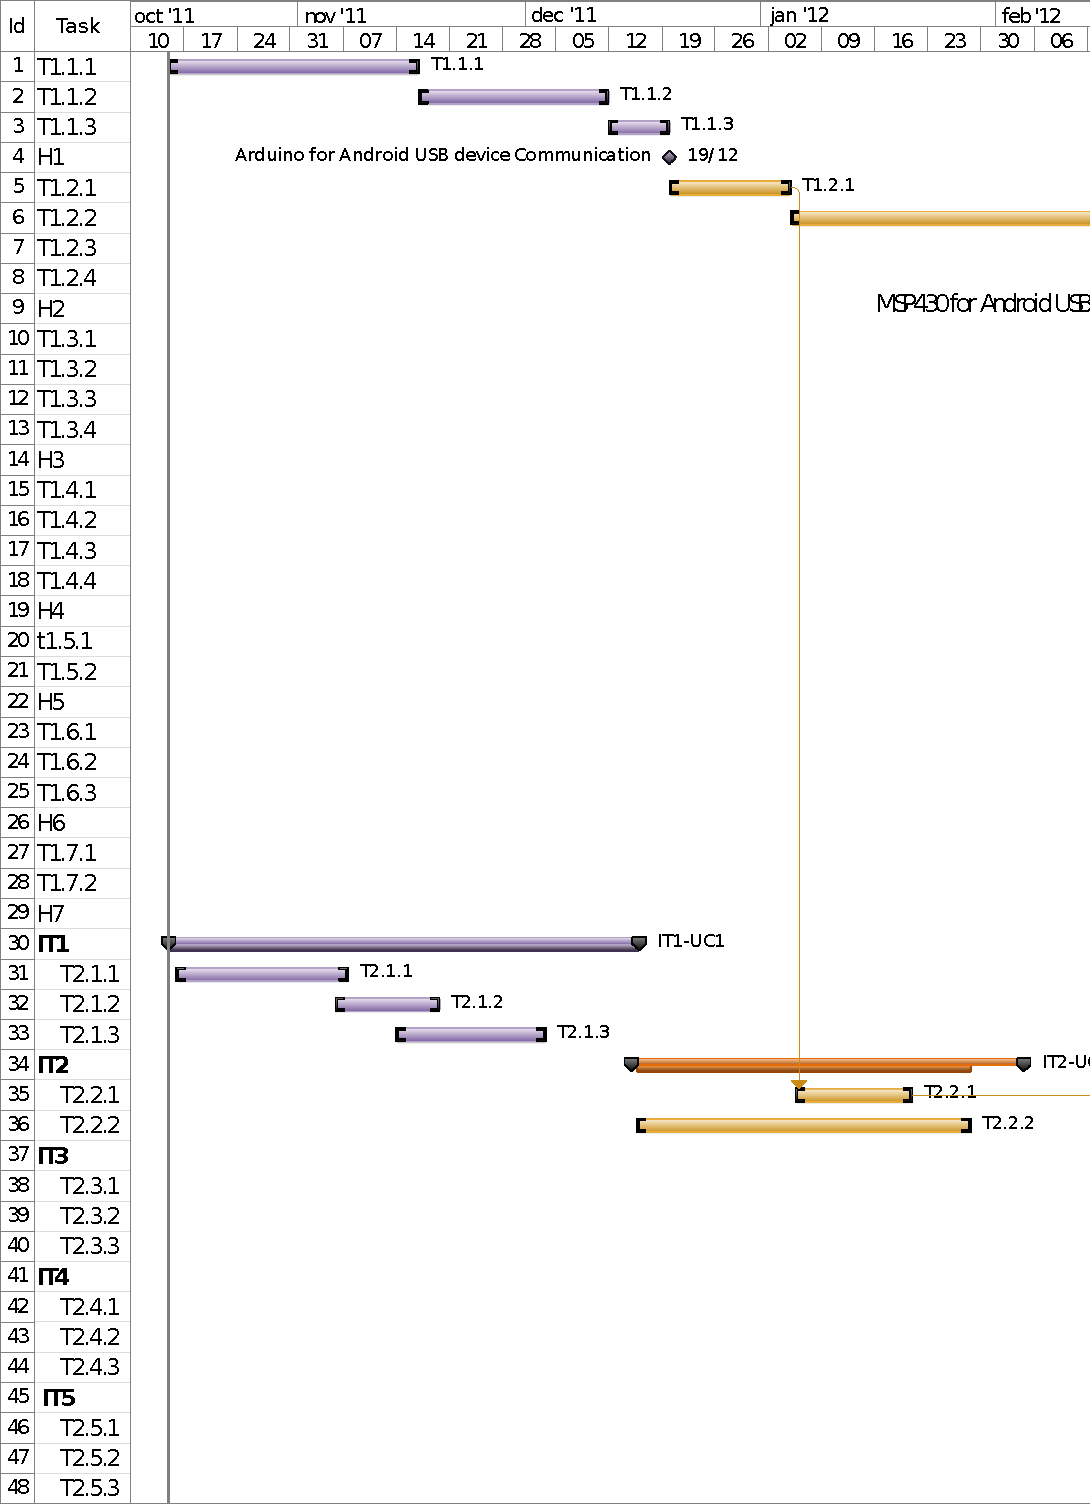
\includegraphics[width=\textwidth]{gantt-l}
		% \label{fig:gantL}
	% \end{figure}
	% \begin{figure}[h]
	 	% \centering
	    	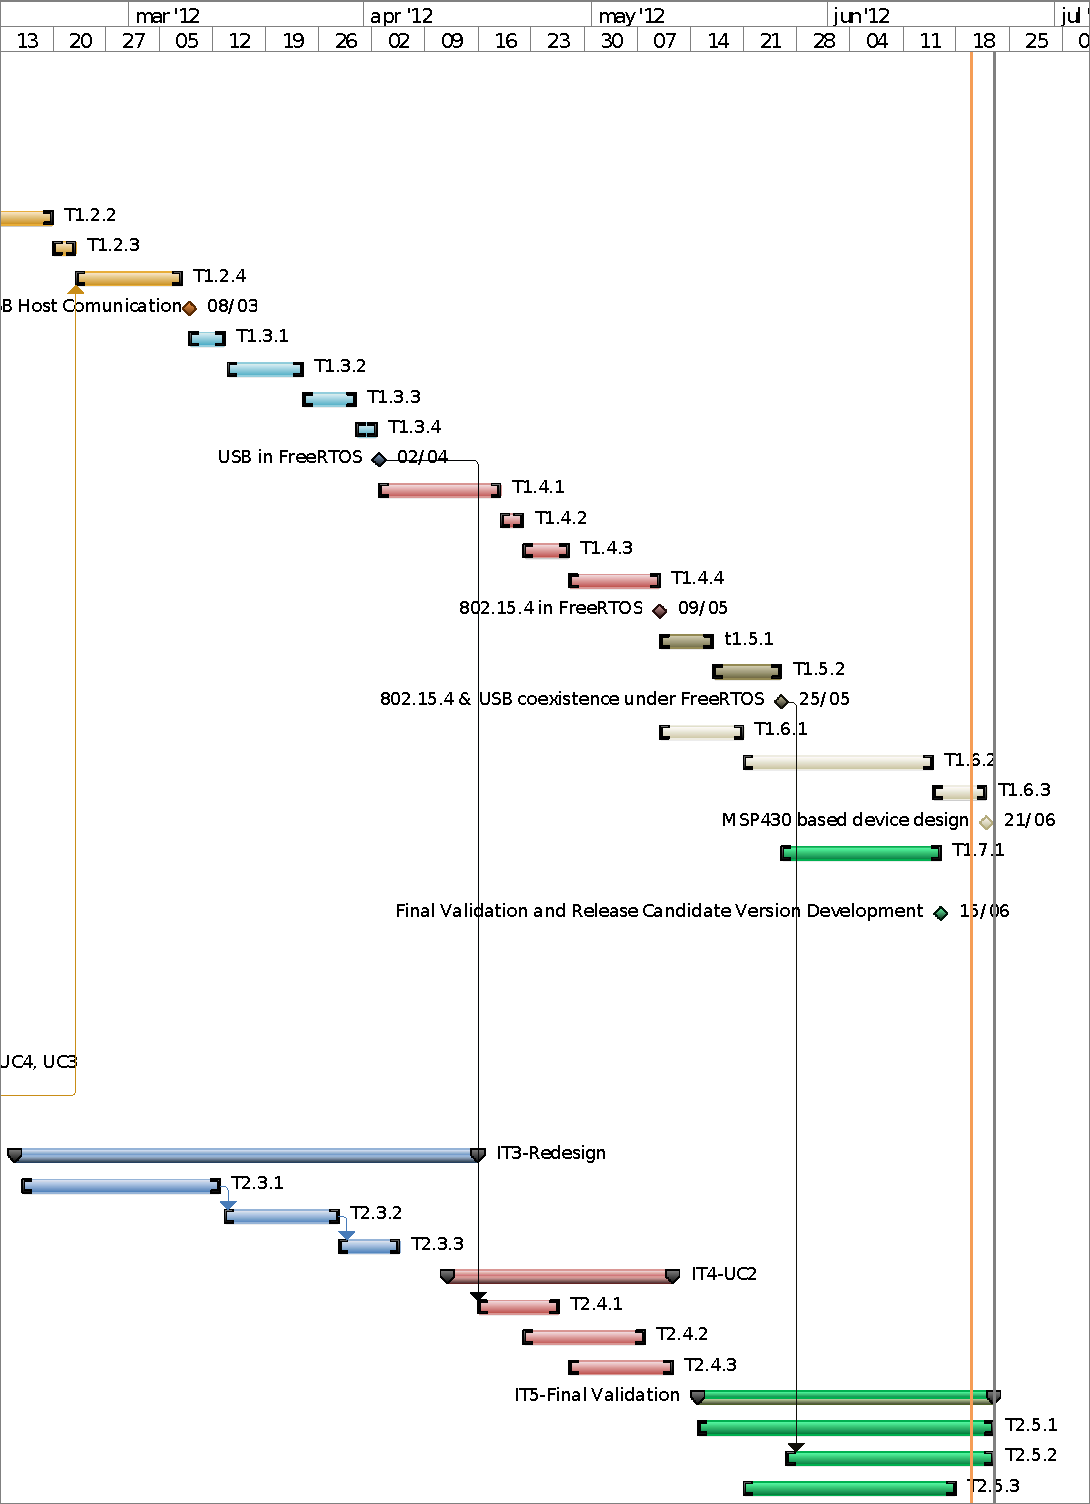
\includegraphics[width=\textwidth]{gantt-r}
		% \label{fig:gantR}
	% \end{figure}

\section{Asset cost}

	% A partir de la planificación anterior, que es la real del proyecto, y considerando que hubo en total cerca de dos meses de vacaciones, podemos considerar que este proyecto tiene una duración de 7 meses con 3 personas trabajando a media jornada. Tipicamente el salario de un ingeniero trabajando en este campo sería de unos 35 euros la hora. Por lo que el coste de un ingeniero durante 7 meses a media jornada sería 35euros/hora * 4 horas/dia * 22 dias/mes * 7 meses = 21560\\
	The total asset cost of the project is presented next, considering the following assumptions:
	\begin{itemize}
		\item The project has been developed through seven months after deducting two months of recess.
		\item Three engineers have been employed halftime through the whole project.
		\item A halftime workday is considered to be of four hours.
		\item The engineer per hour cost considered is 35{\small \euro} per hour.
		\item The ECG delineator node technology is donated and thus does not compute to the price.
	\end{itemize}

	The cost of a single engineer emplyed halftime throughout the seven months is of 35{\small \euro}/hour $\times$ 4 hours/day $\times$ 22 days/month $\times$ 7 months = 21560{\small \euro}.\\

	% Este coste, unido al de los productos que habría habido que adquirir si no hubiera habido nada en el lugar donde se realizase el proyecto nos dan el coste total del proyecto:\\
	The breakdown of the cost of the assets of the project is now exposed.\\

\begin{tabular}{| p{5cm} |l | l | l |} 
\hline
   Name & Number& Price per unit & Total ({\small \euro})\\ \hline
   Motorola Xoom - Wifi & 1 & 399 & 399\\ \hline
   Google ADK & 1 & 70,8 & 70,8\\ \hline
   Exp430F5438 + MSP430F5438A & 1 & 117,89 & 117,89\\ \hline
   TS430PZ100USB + 2xMSP430F6638 & 1 & 60 & 60\\ \hline
   CC2420 & 1 & 4,00 & 4,00\\ \hline
   Prototype & 1 & 38,60 & 38,60\\ \hline
   Final product & 1 & 42,229 & 42,229\\ \hline
   Engineer & 3 & 21560 & 64680\\ \hline
   Total & & & 65392,13\\ \hline
\end{tabular}\\\\

	The total cost of the development of the project rises to 65392,13{\small \euro}. 

\chapter{Product Cost}
\label{ch:cost}

	% El coste de fabricar un dispositivo de manera individual, que es lo que se ha hecho durante el proyecto es el siguiente:\\
	The cost of the production of both a single unit of the final board and an estimated mass production in batches of 10000 (ten thousand) units is as follows.\\

	In this project a single unit of the board has been produced, with the following, exact, cost.\\

\begin{tabular}{| c |l | l | l | l |} 
	\hline
		Name & Reference & Number & Price per unit & Total price\\ \hline
		SMT & 1022311 & 2 & 1,96 & 3,92\\ \hline
		Resistor & 1738981 & 2 & 0,062 & 0,124\\ \hline
		LED & 1699413 & 1 & 0,28 & 0,28\\ \hline
		Capacitor & 1833863 & 6 & 0,03 & 0,18\\ \hline
		Capacitor & 1740650 & 2 & 0,154 & 0,308\\ \hline
		Capacitor & 499110 & 2 & 0,114 & 0,228\\ \hline
		Resistor & 1469918 & 1 & 0,038 & 0,038\\ \hline
		Capacitor & 1833865 & 2 & 0,144 & 0,288\\ \hline
		Diode & 1469389 & 3 & 0,099 & 0,297\\ \hline
	   	Capacitor & 1833803 & 1 & 0,085 & 0,085\\ \hline
 		Capacitor & 1327699 & 1 & 0,36 & 0,36 \\ \hline
  		Resistor & 1500615 & 4 & 0,028 & 0,112\\ \hline
	 	Capacitor & 644183 & 1 & 0,27 & 0,27 \\ \hline
\end{tabular}\\
\begin{tabular}{| c |l | l | l | l |} 
		\hline
		Name & Reference & Number & Price per unit & Total price\\ \hline
	 	Capacitor & 1740632 & 1 & 0,062 & 0,062\\ \hline
	 	MSP430F6638 & 2070274 & 1 & 18,49 & 18,49\\ \hline
	 	Capacitor & 1833888 & 1 & 0,163 & 0,163\\ \hline
	 	Capacitor & 499160 & 2 & 0,122 & 0,244\\ \hline
	 	ESD protection & 1269406 & 1 & 0,63 & 0,63\\ \hline
	 	Microcrystal & 1539364 & 1 & 2,19 & 2,19\\ \hline
	 	Capacitor & 1658880 & 2 & 1,98 & 3,96\\ \hline
	 	%MGRID & 1756749 & 8 & 0,057 & 0,456\\ \hline NO VAN EN EL PRODUCTO
	 	%Header & 7472285 & 1 & 1,34 & 1,34\\ \hline NO VAN EN EL PRODUCTO
	 	%Milligrid & 511031 & 1 & 0,163 & 0,163\\ \hline NO VAN EN EL PRODUCTO
	 	Radio & From TI & 1 & 4,00 & 4,00\\ \hline
		Production & & 1 & 6,00 & 6,00\\ \hline
	 	Total &  &  &  & 42,229\\ \hline
\end{tabular}\\

	The resulting cost of the device is of 42,229{\small \euro}.\\

	%Como todo producto hardware, el precio por unidad suele ser muy elevado pero a partir de cantidades de producción algo más levadas se reduce sustancialmente, para 
	%ilustrarlo este sería el coste de 10000 unidades:\\
	In a mass production scenario the cost of the individual unit is reduced, and an estimation of this is now presented.\\

\begin{tabular}{| c |l | l | l | l |} 
	\hline
		Name & Reference & Number & Price per unit & Total price\\ \hline
		SMT & 1022311 & 20000 & 1,65 & 33000\\ \hline
		Resistor & 1738981 & 20000 & 0,017 & 340\\ \hline
		LED & 1699413 & 10000 & 0,156 & 1560\\ \hline
		Capacitor & 1833863 & 60000 & 0,005 & 300\\ \hline
		Capacitor & 1740650 & 20000 & 0,032 & 640\\ \hline
		Capacitor & 499110 & 20000 & 0,024 & 240\\ \hline
		Resistor & 1469918 & 10000 & 0,01 & 100\\ \hline
		Capacitor & 1833865 & 20000 & 0,024  & 480\\ \hline
		Diode & 1469389 & 30000 & 0,053 & 1590\\ \hline
	   	Capacitor & 1833803 & 10000 & 0,025 & 250\\ \hline
 		Capacitor & 1327699 & 10000 & 0,063 & 630 \\ \hline
  		Resistor & 1500615 & 40000 & 0,021 & 840\\ \hline
	 	Capacitor & 644183 & 10000 & 0,159 & 1590 \\ \hline
\end{tabular}\\\\
\begin{tabular}{| c |l | l | l | l |} 
		\hline
		Name & Reference & Number & Price per unit & Total price\\ \hline
	 	Capacitor & 1740632 & 10000 & 0,012  & 120\\ \hline
	 	MSP430F6638 & 2070274 & 10000 & 13,07 & 130700\\ \hline
	 	Capacitor & 1833888 & 10000 & 0,026  & 260\\ \hline
	 	Capacitor & 499160 & 20000 & 0,041  & 820\\ \hline
	 	ESD protection & 1269406 & 10000 & 0,42  & 4200\\ \hline
	 	Microcrystal & 1539364 & 10000 & 1,40 & 14000\\ \hline
	 	Capacitor & 1658880 & 20000 & 1,03  & 20600\\ \hline
	 	%MGRID & 1756749 & 80000 & 0,043  & 0,456\\ \hline NO VAN EN EL PRODUCTO
	 	%Header & 7472285 & 10000 & 1,34 & 1,34\\ \hline NO VAN EN EL PRODUCTO
	 	%Milligrid & 511031 & 10000 & 0,163 & 0,163\\ \hline NO VAN EN EL PRODUCTO
	 	Radio & From TI & 10000 & 4,00 & 40000\\ \hline
		Base board &  & 1 & 100 & 100\\ \hline
		Production &  & 10000 & 0.05 & 500\\ \hline
	 	Total &  &  &  & 252860\\ \hline
	 	Total per unit &  &  &  & 25,286\\
	\hline
\end{tabular}\\\\

	The cost of the device produced in batches of 10000 (ten thousand) units is reduced to 25,286{\small \euro}.